\section{Existence of Drawings with Circular Arcs}
\label{sect:existence-of-drawings-with-circular-arcs}

For an arbitrary set of edge-disjoint paths ${\Pi = \left\lbrace P_1, \ldots, P_k \right\rbrace}$ the existence of a drawing of ${\Pi}$ with circular arcs is not guaranteed.

A circle \emdash or circular arc for that matter \emdash is uniquely determined by three distinct points. If two paths ${P_i \neq P_j}$ were to have three or more vertices in common, the circular arcs used to draw them would intersect in at least three points and would therefore overlap. However, in \cref{thm:necessary-condition-not-sufficient} we show that the resulting necessary condition of two paths ${P_i \neq P_j}$ having at most two vertices in common is not sufficient in guaranteeing the existence of a (valid) drawing of ${\Pi}$ with circular arcs. We start by showing the following lemma:

\hfill



\begin{lemma}
\label{thm:existence-without-touches}
A drawing of ${\Pi}$ with circular arcs in which edges touch in non-endpoints can be transformed into a drawing of ${\Pi}$ with circular arcs in which said edges either cross or do not intersect at all.
\end{lemma}

\begin{proof}
When two edges touch in non-endpoints, then so do the paths they are part of and the circular arcs used to draw these paths. Adjusting the curvature of one of said circular arcs by an infinitesimal amount causes these circular arcs to either cross or to not intersect at all.

Considering this adjustment does not alter the ordering of vertices on said circular arc, it is only left to show that this adjustment can be performed such that the resulting circular arc does not overlap other circular arcs, or intersect vertices not part of the respective path. There's a finite number of vertices and paths in a drawing of ${\Pi}$ with circular arcs; hence this adjustment can indeed be performed without violating any of the constraints imposed by ${\Pi}$.
\end{proof}





\clearpage

\begin{theorem}
\label{thm:necessary-condition-not-sufficient}
There exists a set of edge-disjoint paths ${\Pi}$ in which any two paths have at most two vertices in common, \ie{} ${\forall i \neq j \colon \abs{V(P_i) \cap V(P_j)} \leq 2}$, for which no (valid) drawing with circular arcs exists.
\end{theorem}

\begin{proof}
An arrangement of pseudocircles is a finite list ${\mathcal{C} = (c_1, \ldots, c_n)}$ of Jordan curves in the plane, such that \begin{enumerate*}[label=(\roman*)] \item every two curves intersect in at most two points, and \item if two curves meet in a point, they cross in said point \end{enumerate*}. Two arrangements are said to be \emph{equivalent} if there exists a homeomorphism from the plane onto itself that transforms one of the arrangements into the other one. An arrangement of pseudocircles is said to be \emph{circleable} if it is equivalent to an arrangement of proper circles \cite{Kang}.

Linhart and Ortner \cite{Linhart} showed that the arrangement of pseudocircles in \cref{fig:non-circleable-arrangement-of-pseudocircles} is not circleable.

\begin{figure}[H]
  \centering
  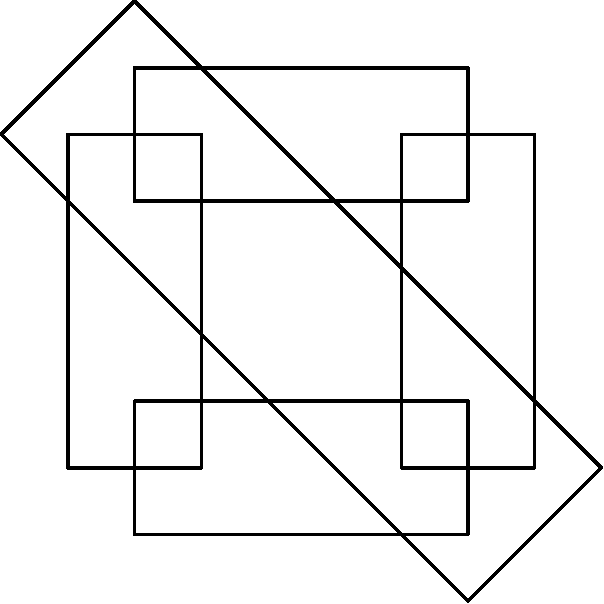
\includegraphics[width=0.4\textwidth]{Resources/Figures/Arrangement-of-Pseudocircles.pdf}
  \quad
  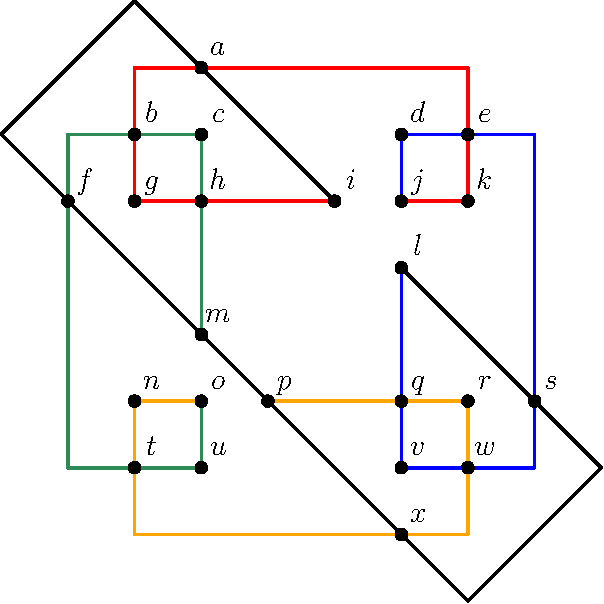
\includegraphics[width=0.4\textwidth]{Resources/Figures/Arrangement-of-Pseudoarcs.pdf}
  \caption{An arrangement of pseudocircles that is not circleable (left) and a derived arrangement of pseudo circular arcs (right).}
  \label{fig:non-circleable-arrangement-of-pseudocircles}
\end{figure}

\noindent
Let us choose a set of edge-disjoint paths ${\Pi = \lbrace P_1, \ldots, P_n \rbrace}$ such that each path represents one of the pseudocircles in \cref{fig:non-circleable-arrangement-of-pseudocircles} and their shared vertices completely encode all of said pseudocircles' intersections with each other. A possible choice would be ${P_1 = \mathit{ihgbaekj}}$ (red), ${P_2 = \mathit{pqrwxtno}}$ (yellow), ${P_3 = \mathit{mhcbftuo}}$ (green), ${P_4 = \mathit{lqvwsedj}}$ (blue), and ${P_5 = \mathit{iafmpxsl}}$ (black).

Considering circular arcs are slices of complete circles and the arrangement of pseudocircles in \cref{fig:non-circleable-arrangement-of-pseudocircles} is not circleable, a drawing of ${\Pi}$ with circular arcs in which no two circular arcs touch in non-endpoints can not exist. \Cref{thm:existence-without-touches} then shows that in fact, no drawing of ${\Pi}$ with circular arcs can exist at all.
\end{proof}





\clearpage

\noindent
\Cref{thm:necessary-condition-not-sufficient} shows that the trivial condition of two paths having at most two vertices in common is not sufficient in guaranteeing the existence of a (valid) drawing of ${\Pi}$ with circular arcs. Let us now be a little more restrictive and instead consider an ordered sequence of edge-disjoint paths ${\Pi = (P_1, \ldots, P_k)}$ in which none of a path ${P_i}$'s internal vertices are contained in an earlier path, \ie{} a path ${P_j}$ with ${j < i}$:
%
\begin{equation}
  V_\text{int}(P_i) \cap V(P_1 \cup \ldots \cup P_{i-1}) \stackrel{!}{=} \varnothing,
  \quad i = 2 \ldots k
  \label{eqn:blah-blah-property}
\end{equation}





\hfill

\begin{theorem}
\label{thm:existence-of-drawing}
An ordered sequence of edge-disjoint paths ${\Pi = (P_1, \ldots, P_k)}$ fulfilling \cref{eqn:blah-blah-property} permits a drawing of ${\Pi}$ with circular arcs.
\end{theorem}

\begin{proof}
We will provide a method to construct a drawing of ${\Pi}$ with circular arcs by sequentially drawing the paths ${P \in \Pi}$ in their designated order.

\Cref{eqn:blah-blah-property} ensures that, when drawing a path ${P = (v_1, \ldots, v_n)}$, its internal vertices ${v_2, \ldots, v_{n-1}}$ have not yet been drawn. Since the paths are edge-disjoint, its edges have not yet been drawn either. In case an endpoint of ${P}$ has not yet been drawn, we can assign it an arbitrary position, as long as it is not on any of the circular arcs that have already been drawn.

Considering there's a finite number of vertices and edges, there exists a circular arc ${\Gamma_P}$ between ${P}$'s endpoints that neither intersects any of the vertices that have already been drawn (other than said endpoints), nor overlaps any circular arc that has already been drawn.

It is possible, however, for ${\Gamma_P}$ to intersect other circular arcs. Drawing one of ${P}$'s internal vertices on such an intersection would visually introduce new edges, rendering the drawing of ${\Pi}$ invalid. Considering a pair of non-overlapping circular arcs intersects in at most two points, the number of points on ${\Gamma_P}$ on which we can not draw ${P}$'s internal vertices is finite, and there are infinitely many points left on which said vertices could be drawn without rendering the drawing invalid. Therefore we can draw ${P}$'s internal vertices, in order, on the circular arc and thereby partition ${\Gamma_P}$ into smaller circular arcs ${\Gamma_e}$ representing the individual edges ${e \in E(P)}$.
\end{proof}





\hfill

\noindent
We have seen that an ordered sequence of edge-disjoint paths ${\Pi = (P_1, \ldots, P_k)}$ fulfilling \cref{eqn:blah-blah-property} permits a (greedy) drawing of ${\Pi}$ with circular arcs. Therefore we shall also refer to ${\Pi}$ as a \emph{greedily realizable sequence of paths}. Vertices ${v \in V(\Pi)}$ shall be said to be \emph{laid out} by the first path, \ie{} the path ${P_i \in \Pi}$ with the lowest index ${i}$, in which they occur. If ${v}$ is internal to said path, it shall be called \emph{constrained} (with respect to ${\Pi}$); otherwise, it shall be called \emph{unconstrained} (with respect to ${\Pi}$). The constrained and unconstrained vertices form the sets ${V_\text{c}(\Pi)}$ and ${V_\text{u}(\Pi)}$, respectively. Obviously ${V_\text{c}(\Pi) \cap V_\text{u}(\Pi) = \varnothing}$ and ${V_\text{c}(\Pi) \cup V_\text{u}(\Pi) = V(\Pi)}$.

Note that there are definitely other properties guaranteeing the existence of a (valid) drawing of ${\Pi}$ with circular arcs \emdash possibly even less restrictive ones. We use this one because it suggests a straight-forward method to create a drawing, as illustrated in the proof of \cref{thm:existence-of-drawing}.
